%!TEX root = ../../main.tex

\chapter{Das Monty-Hall-Problem - Einführung}

Das Monty-Hall-Problem ist Statistikern als Paradoxon in der Elementarwahrscheinlichkeitstheorie bekannt. Es geht dabei um die Frage, ob eine Wahl, die zunächst 
zufällig unter drei a priori \footnote[1]{Wahrscheinlichkeit zu Beginn} gleich wahrscheinlichen Möglichkeiten getroffen wurde, geändert werden sollte, wenn zusätzliche 
Informationen enthüllt werden. Die Aufgabe ist ursprünglich aus der von Monty Hall modertierten Spielshow "Lets Make a Deal" abzuleiten. Sie fand ihren Anfang 
1963 und ihr Ende 1977. In jeder Folge spielte der Host der Spielshow, Monty Hall, Spiele mit seinem Publikum. Diese Spiele variierten stark, jedoch war das Grundprinzip
häufig das Selbe. Spieler aus dem Publikum mussten sich zwischen garantierten, kleinen Gewinnen und eventuellen, durch "Glückspiel" gewonnene, große Preise, entscheiden.
In einer der Folgen, die häufig als die Klimax der Show beschrieben wird, wurde den Spielern aus dem Publikum drei identische Türen gezeigt. Hinter diesen drei 
identischen Türen befinden sich die potenziellen Gewinne, wovon zwei Gewinne Ziegen waren. Hinter der dritten Tür war jedoch der Hauptgewinn, ein neues Auto.

Das Spiel konnte beginnen. Der Ablauf war nicht immer gleich. Ursprünglich entschied sich der Spieler für eine Tür, welche er allerdings noch nicht öffnete.
Der Host gibt dem Spieler die Möglichkeit, seine Entscheidung zu ändern, sofern dieser es wünscht. der Spieler entscheidet sich für eine Tür, welche jedoch nicht geöffnet wird. Dann öffnet der Host eine Tür für
den Spieler, von der er sicher weiß, dass sich eine Ziege dahinter befindet.


% \begin{figure}[h]
% \centering
% 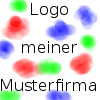
\includegraphics[height=.8\textwidth]{logo.png}
% \caption{Das Logo der Musterfirma\footnotemark}
% \end{figure}



%\begin{wrapfigure}{r}{.4\textwidth}
%\centering
%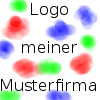
\includegraphics[height=.35\textwidth]{logo.png}
%\vspace{-15pt}
%\caption{Das Logo der Musterfirma\footnotemark}
%\end{wrapfigure}
%Quelle muss in Fußnote stehen (da sonst aufgrund eines Fehlers nicht kompiliert
% wird)
\footnotetext{aus \cite{mustermann:2012}}


% \begin{equation}
% t-t_{0}=\sqrt{\frac{l}{g}}\int_{0}^{\varphi}{\frac{d\psi}{\sqrt{1-k^{2}\sin^{2} {\psi}}}} = \sqrt{\frac{l}{g}} F(k,\varphi)
% \label{xyz}
% \end{equation}

% \begin{itemize}
% \item Dies ist der erste Punkt, der aufgeführt wird.
% \item Dies ist der zweite Punkt, der aufgeführt wird. Manchmal will man auch etwas \textbf{fett} oder \textit{kursiv} oder \textbf{\textit{beides in Kombination}}  drucken.
% \item Dies ist der dritte Punkt, der aufgeführt wird.
% \end{itemize}

